% !TEX TS-program = pdflatex
% !TEX encoding = UTF-8 Unicode
% arara: xelatex
% arara: bibtex
% arara: xelatex
\documentclass[11pt,a4paper]{bidimoderncv}
% M.Amintoosi
% ORCID: 0000-0001-9640-6475  
\usepackage[numbers]{natbib}%
\hypersetup{pdfauthor=Mahmood Amintoosi, pdfcreator=Hakim Sabzevari University}

\cvtheme[blue]{bidiclassic}%casual} 
\usepackage{tikz}
\usetikzlibrary{tikzmark}
%\usepackage{enumitem}
\usepackage{pifont}
\usepackage{xepersian}
%\settextfont[BoldFont={IRLotusICEE_Bold.ttf}, BoldItalicFont={IRLotusICEE_BoldIranic.ttf}, ItalicFont={IRLotusICEE_Iranic.ttf},Scale=1.2]{IRLotusICEE.ttf}%{IRZar.ttf}
\settextfont[Scale=1.2]{IRLotusICEE}%{IRZar.ttf}


%\setlatintextfont[Scale=1]{Linux Libertine}%{Times New Roman}%
\defpersianfont\mytitlefont[Scale=.8]{IRTitr}%{XB Zar Bold}%{XB Kayhan Sayeh}

\AtBeginDocument{\recomputelengths} 
\firstname{\mytitlefont محمود}
\familyname{\mytitlefont امین‌طوسی\hspace*{10mm}}%\newline\hspace*{10mm}
\resumename{رزومه}
\title{%\large
دانشیار علوم کامپیوتر،
\newline
 دانشگاه فردوسی مشهد 
\newline \large
(مامور از دانشگاه حکیم سبزواری)}
\address{خراسان رضوی، مشهد، \\دانشگاه فردوسی، \\دانشکده علوم ریاضی\\
طبقه دوم، اتاق ۷۱۶ }   
\mobile{۰۹۱۲۲۸۷۴۶۹۴}
\phone{۰۵۱۳۸۸۰۵۶۷۸}  
%\fax{شماره فکس}                          
\email{m.amintoosi@\{um.ac.ir,gmail\}}
\extrainfo{\httplink[http://mamintoosi.ir]{mamintoosi.ir}} 
\photo[100pt]{mAmintoosi_1400.jpg}                         
%\quote{نقل قول}  
\begin{document}

\begin{tikzpicture}[remember picture,overlay]
\fill[blue!5]
  (current page.north west) rectangle ([yshift=-4cm]current page.east|-{pic cs:end});
\end{tikzpicture}

\maketitle

%\setlength{\hintscolumnwidth}{0.1\textwidth}

\vspace{-10mm}
\section{وضعیت کاری}
\cventry{۱۳۷۷-۱۳۸۰}{حق‌التدریس}{گروه ریاضی، دانشگاه تربیت معلم سبزوار (حکیم سبزواری)}{}{}{}
\cventry{1380 - 1401}{عضو هیأت علمی}{دانشکده ریاضی و علوم کامپیوتر، دانشگاه حکیم سبزواری}{}{}{}
\cventry{1390-1393}{مدیر فناوری}{دانشگاه حکیم سبزواری}{}{}{}
\cventry{1401 - تاکنون}{عضو هیأت علمی}
{دانشکده علوم ریاضی، دانشگاه فردوسی  مشهد}{}{}{}

\section{تحصیلات}
\cventry{۱۳۷۰-۱۳۷۴}{کارشناسی}{دانشگاه فردوسی}{ مشهد}{}{ریاضی (کاربرد در کامپیوتر)}  
\cventry{۱۳۷۵-۱۳۷۸}{کارشناسی ارشد}{دانشگاه فردوسی}{ مشهد}{}{مهندسی کامپیوتر(نرم افزار)}  
\cventry{۱۳۸۴-۱۳۸۹}{دکترا}{دانشگاه علم و صنعت ایران}{ تهران}{}{مهندسی کامپیوتر (هوش مصنوعی) - پردازش تصویر}  

\section{سابقه تدریس}
\cvlistitem	{تدریس دروس کامپیوتر از سال 1376 در دانشگاههای مختلف}
\subsection{دروس تدریس شده:}
\cvlistdoubleitem[\Neutral]{مبانی کامپیوتر و برنامه‌سازی}{برنامه‌سازی پیشرفته}
\cvlistdoubleitem[\Neutral]{ساختمان داده‌ها}{محیط‌های چندرسانه‌ای}
\cvlistdoubleitem[\Neutral]{طراحی الگوریتم‌ها}{آشنایی با نرم‌افزار \lr{MATLAB}}
\cvlistdoubleitem[\Neutral]{گرافیک کامپیوتری}{سیستم عامل }
\cvlistdoubleitem[\Neutral]{ساختمان و زبان ماشین}{پایگاه داده‌ها}
\cvlistdoubleitem[\Neutral]{طراحی و پیاده‌سازی زبانهای برنامه‌سازی}{محاسبات نرم}
\cvlistdoubleitem[\Neutral]{بهینه‌سازی ترکیبیاتی}{هوش مصنوعی }
\cvlistdoubleitem[\Neutral]{یادگیری ماشین}{داده‌کاوی }
\cvlistdoubleitem[\Neutral]{مبانی پردازش تصویر}{آشنایی با نرم‌افزار \lr{\LaTeX}}
\cvlistdoubleitem[\Neutral]{بازیابی اطلاعات}{یادگیری عمیق}
\cvlistdoubleitem[\Neutral]{متن‌کاوی و وب‌کاوی}{داده‌کاوی محاسباتی }

\newpage
\section{موضوعات کاری}
\cvlistdoubleitem[\ding{72}\ding{72}\ding{78}]
{بینایی ماشین}% \lr{\small(Machine Vision)}}
{یادگیری عمیق }
%\lr{{\small 
%}}}
\cvlistdoubleitem[\ding{72}\ding{77}\ding{73}]{یادگیری ماشین}
%\lr{\small (Machine Learning)}}
{داده‌کاوی}
%\cvlistdoubleitem[\ding{72}\ding{78}\ding{73}]{بازسازی سه‌بعدی \lr{\small (3D-Reconstruction)}}{پایدارسازی \lr{\small (Stabilization)}}
\cvlistdoubleitem[\ding{72}\ding{76}\ding{73}]{بهینه‌سازی ترکیبیاتی}{پردازش تصویر}%\lr{\small Seam Carving}}
%\cvlistdoubleitem[\ding{72}\ding{73}\ding{73}]{یادگیری ماشین \lr{\small (Machine Learning)}}{شناسائی آماری الگو}
%\cvlistdoubleitem[\ding{72}\ding{77}\ding{73}]{ترکیب تصاویر \lr{\small (Fusion)}}{تصاویر عریض \lr{\small (Panorama)}}
%\cvlistdoubleitem[\ding{72}\ding{73}\ding{73}\ding{73}]{مسائل معکوس}{فیلترهای وفقی}

\section{طرح‌های پژوهشی}
\cvlistitem  {آشکار سازی رگ های خونی شبکیه چشم با روشهای درهم تنیدگی تصویر\hfill {\small\em  پایان یافته}}
\cvlistitem  {طراحی و پیاده سازی قالب زی‌پرشین پایان‌نامه‌های دانشگاه حکیم سبزواری\hfill {\small\em  پایان یافته}}
\cvlistitem  {طراحی و پیاده سازی وب سایت دانشگاه حکیم سبزواری\hfill {\small\em پایان یافته}}
\cvlistitem  {خودكارسازی برنامه ریزی هفتگی دروس دانشگاهی\hfill {\small\em پایان یافته}}
\cvlistitem  {طراحی و پیاده سازی برنامه مورد نیاز دفتر نظارت و ارزیابی دانشگاه حکیم سبزواری\hfill {\small\em پایان یافته}}
%\cvlistitem  {خوشه‌بندی بر مبنای رفتار گروه ماهی‌ها\hfill {\small\em در حال داوری}}
%\cvlistitem  {رمزنگاری بصری\hfill {\small\em در حال داوری}}

 

\section{سخنرانی‌ها و کارگاههای برگزار شده}
\cvline{۱۴۰۱}{ سخنرانی با موضوع شبکه‌های عصبی پیچشی گراف، {\small دانشگاه فردوسی مشهد}، \httplink[لینک اسلایدها]{https://mamintoosi.github.io/slides/topics/GNN/GNN-2022.html}:\newline\footnotesize
\url{{https://mamintoosi.github.io/slides/topics/GNN/GNN-2022.html}}}
\cvline{۱۴۰۰}{ کارگاه یادگیری عمیق با
\lr{PyTorch}، {\small دانشگاه حکیم سبزواری}، \httplink[لینک اسلایدها]{https://mamintoosi.github.io/slides/topics/DL-HSU/DeepLearning-Workshop-ESLA2022.html}:\newline\footnotesize
\url{{https://mamintoosi.github.io/slides/topics/DL-HSU/DeepLearning-Workshop-ESLA2022.html}}}
\cvline{۱۳۹۸}{ کارگاه یادگیری عمیق با
\lr{TensorFlow}، {\small دانشگاه حکیم سبزواری}، \httplink[اسلایدها در گیت‌هاب]{https://mamintoosi.github.io/slides/topics/DL-HSU-Fall2019/DeepLearning-Workshop-TSCO2019.html}
%\newline\footnotesize
%\url{https://mamintoosi.github.io/slides/topics/DL-HSU-Fall2019/DeepLearning-Workshop-TSCO2019.html}
}
\cvline{۱۳۹۸}{سخنرانی با موضوع بازی ‌های ریاضی و کامپیوتر، {\small دانشگاه حکیم سبزواری}}
\cvline{۱۳۹۵}{سخنرانی با موضوع یادگیری ماشین، {\small دانشکده فنی حرفه‌ای دختران سبزواری}}
\cvline{۱۳۹۳}{سخنرانی با موضوع معرفی رشته علوم تصمیم و مهندسی دانش ، {\small دانشگاه حکیم سبزواری}}
\cvline{۱۳۹۲}{کارگاه آشنایی با نرم‌افزار حروف‌چینی لاتک و بستهٔ زی‌پرشین، {\small هشتمین کنفرانس بینایی ماشین و پردازش تصویر ایران، دانشگاه زنجان}}
\cvline{۱۳۹۲}{سخنرانی با موضوع بهینه‌سازی در پردازش تصویر ، {\small دانشگاه حکیم سبزواری}}
\cvline{۱۳۹۲}{سخنرانی با موضوع ثبت تصویر ، {\small دانشگاه حکیم سبزواری}}
\cvline{۱۳۹۰}{کارگاه آشنایی با نرم‌افزار حروف‌چینی لاتک و بستهٔ زی‌پرشین، {\small۲۲ومین سمینار جبر ایران}}
\cvline{۱۳۹۰}{کارگاه آشنایی با نرم‌افزار حروف‌چینی لاتک و بستهٔ زی‌پرشین، {\small دانشگاه علم و صنعت ایران}}
%\cvline{۱۳۹۰}{سخنرانی با موضوع هوش مصنوعی ، {\small دانشگاه پیام نور تربت حیدریه}}
\cvline{۱۳۹۰}{کارگاه آشنایی با نرم‌افزار حروف‌چینی لاتک و بستهٔ زی‌پرشین، {\small هفتمین کنفرانس بینایی ماشین و پردازش تصویر ایران}}
\cvline{۱۳۹۰}{کارگاه آشنایی با نرم‌افزار حروف‌چینی لاتک و بستهٔ زی‌پرشین، {\small۴۲ومین کنفرانس ریاضی ایران}}
\cvline{۱۳۸۹}{کارگاه آشنایی با نرم‌افزار حروف‌چینی لاتک و بستهٔ زی‌پرشین، {\small دانشگاه حکیم سبزواری}}
\cvline{۱۳۸۷}{عصر اطلاعات و اینترنت، {\small جلسهٔ دبیران ریاضی کاشمر}}
\cvline{۱۳۸۶}{مروری بر پروژ‌ه‌های انجام شده در حوزهٔ پردازش تصاویر و مرتبط با ترافیک، {\small هشتمین کنفرانس ترافیک و مهندسی حمل و نقل}}
\cvline{۱۳۸۳}{دوره آموزشی طراحی صفحات وب جهت اعضای هیات علمی، {\small دانشگاه حکیم سبزواری}}
\cvline{۱۳۸۲}{بهینه‌سازی با روش اجتماع مورچگان، {\small دانشگاه حکیم سبزواری}}
\cvline{۱۳۸۱}{محاسبه با \lr{DNA}، {\small دانشگاه حکیم سبزواری}}
%\cvline{۱۳۸۱}{دوره آموزشی اینترنت جهت اعضای هیات علمی، {\small دانشگاه حکیم سبزواری}}
\cvline{۱۳۸۰}{مروری بر الگوریتم‌های ژنتیک، {\small دانشگاه حکیم سبزواری}}
\cvline{1379}{دوره آموزشی ویندوز جهت کارکنان شرکت برق، {\small شهرستان سبزوار}}


%\newpage 
\section{تجربیات و مهارت‌ها در زبانهای برنامه‌نویسی، نرم‌افزارها و بسته‌ها}
%\cvline{}{در زمینهٔ زبانهای برنامه‌نویسی و نرم‌افزارهای زیر تجربیاتی دارم:}
%\cvline{زبانهای برنامه‌نویسی، نرم‌افزارها، بسته‌ها}{}
\begin{flushleft}
\begin{latin}
{FORTRAN, BASIC, COBOL, FoxPro, C and C++, Assembly, Pascal, SQL, PHP, Perl, Java and Java Script, Python, Visual Studio Code, Google colab, Github,
 MATLAB, C++ Builder, Delphi, \LaTeX, Microsoft Office (Word, Excel, Access, OneNote, Visio,
 OutLook, PowerPoint), Visual SVN, TortoiseSVN, WinEdt, TeXMaker, Notepad++,\XePersian, 
 Farsi\TeX, Bib\TeX, NetBeans, MiKTeX, JACK, GPSS and Some Others.}
\end{latin}
\end{flushleft}
%\cvline{نرم‌افزارها و بسته‌ها}{}

%\newpage
\section{عضویت در گروه‌ها}
\begin{latin}
\small
%\begin{flushleft}
%\setlist{nosep}
%\setlength\labelsep{\dimexpr\labelsep + 0.5em\relax}
%\setlength\leftmargini{\dimexpr\leftmargini + 0.5em\relax}
\begin{itemize}%[label={• }]	
\item Member of the Iranian Society of Machine Vision and Image Processing.	\hfill {\scriptsize\em http://www.ismvip.ir/}
\item Previous member of the ACM (Association for Computing Machinery)\hfill {\scriptsize\em http://www.acm.org//}
\item Previous member of IEEE (Institute of Electrical and Electronics Engineers). \hfill {\scriptsize\em http://www.ieee.org/}
\item Member of the ParsiLaTeX (Iranian \LaTeX{} usergroup). \hfill {\scriptsize\em http://www.parsilatex.com}
%\item Member of the EURO Working group on Automated TimeTabling (WATT) \hfill {\scriptsize\em http://www.asap.cs.nott.ac.uk/ASAP/watt/}
%\item Member of the EU/ME the European chapter on metaheuristics. \hfill {\scriptsize\em http://143.129.203.3/eume/php/eume.main.php}
%\item Member of the EURO Special Interest Group on Cutting and Packing (ESICUP). \hfill {\scriptsize\em http://www.apdio.pt/sicup/}
\end{itemize}	
%{\small • Member of the Iranian Society of Machine Vision and Image Processing. \hfill {\scriptsize\em http://www.ismvip.ir/}}\\
%{\small • Member of the ACM (Association for Computing Machinery) \hfill {\scriptsize\em http://www.acm.org//}}\\
%{\small • Student member of IEEE (Institute of Electrical and Electronics Engineers). \hfill {\scriptsize\em http://www.ieee.org/}}\\
%{\small • Member of the ParsiLaTeX (Iranian \LaTeX{} usergroup). \hfill {\scriptsize\em http://www.parsilatex.com}}\\
%{\small • Member of the EURO Working group on Automated TimeTabling (WATT) \hfill {\scriptsize\em http://www.asap.cs.nott.ac.uk/ASAP/watt/}}\\
%{\small • Member of the EU/ME the European chapter on metaheuristics. \hfill {\scriptsize\em http://143.129.203.3/eume/php/eume.main.php}}\\
%{\small • Member of the EURO Special Interest Group on Cutting and Packing (ESICUP). \hfill {\scriptsize\em http://www.apdio.pt/sicup/}}\\
%{\small • Student member of ISIC (International Student Identification Card). \hfill {\scriptsize\em http://www.isic.ir/}}\\
%{\small • Member of the \LaTeX  Community. \hfill {\scriptsize\em http://www.latex-community.org/}}\\
%\end{flushleft}
\end{latin}

%\newpage

\section{ فعالیت‌های حرفه‌ای}
\cvline{۱۴۰۰-۱۳۹۵}{داوری مقالات در چند کنفرانس و سمینار دانشکده ریاضی و علوم کامپیوتر، دانشگاه حکیم سبزواری}
\cvline{۱۳۹۶}{عضو کمیته علمی \lr{7$^{th}$ International Conference on Computer and Knowledge Engineering (ICCKE 2017)}، دانشگاه فردوسی مشهد}
\cvline{۱۳۹۴}{عضو کمیته علمی و مسئول بخش در هفتمین کنفرانس بین‌المللی فناوری اطلاعات و دانش، دانشگاه ارومیه}
%\lr{The 7th International Conference on Information and Knowledge Technology (IKT 2015)}
\cvline{۱۳۹۳}{عضو کمیته علمی و مسئول بخش در \lr{4$^{th}$ International Conference on Computer and Knowledge Engineering (ICCKE 2014)}، دانشگاه فردوسی مشهد}
\cvline{۱۳۹۳}{داور مقاله در \lr{IEEE Intelligent Transportation Systems Society Conference Management System (ITSC14)}}
\cvline{۱۳۹۲}{داوری مقالات در \lr{Symposium on Artificial Intelligence and Signal Processing (AISP 2013)}}
\cvline{۱۳۹۲}{عضو کمیته علمی \lr{3$^{th}$ International Conference on Computer and Knowledge Engineering (ICCKE 2013)}، دانشگاه فردوسی مشهد}
\cvline{۱۳۹۲}{عضو کمیته علمی هشتمین کنفرانس ماشین بینایی و پردازش تصویر ایران، دانشگاه زنجان}
\cvline{۱۳۹۲}{عضو کمیته اجرایی پانزدهمین کنفرانس ملی شیمی معدنی ایران، دانشگاه حکیم سبزواری}
\cvline{۱۳۹۱}{داور مقالات \lr{2thInternational Conference on Computer and Knowledge Engineering (ICCKE 2012)}، دانشگاه فردوسی مشهد}
\cvline{۱۳۹۱}{عضو کمیته علمی هفتمین کنفرانس ماشین بینایی و پردازش تصویر ایران، دانشگاه علم و صنعت ایران}
\cvline{۱۳۹۰}{عضو کمیته اجرایی بیست و دومین سمینار جبر ایران، دانشگاه حکیم سبزواری}
\cvline{۱۳۹۰}{داور مقالات \lr{International Conference on Computer and Knowledge Engineering (ICCKE 2011)}، دانشگاه فردوسی مشهد}
\cvline{داوری در}{\lr{IET Image Processing Journal, IEEE Trans. on Sys., Man, and Cybernetics}}
\cvline{چند مجله}{\lr{Journal of Artificial Intelligence \& Data Mining,  Signal Processing-Elsevier}}
\cvline{منجمله}{نشریه پردازش علائم و داده ها، ‌هوش محاسباتی در مهندسی برق، نشریة مهندسی برق و مهندسی كامپیوتر ایران و دوفصلنامه فناوری اطلاعات وارتباطات ایران}
%\cvline{}{یکی از مدیران گروه پارسی‌لاتک : \hfill \url{http://www.parsilatex.com}}
%\cvline{}{}
%\cvline{}{}
%\cvline{}{}

%\section{زمینه‌های کاری مورد علاقه}
%\cvline{بینائی ماشین}{\small  به خاطر موضوع پروژه روی موارد مرتبط با آن کار می‌کنم.}
%\cvline{پردازش تصویر}{\small موضوع پروژه مرتبط با این مقوله نیز می‌باشد.}
%\cvline{بهینه‌سازی ترکیبیاتی}{\small پروژهٔ کارشناسی ارشد اینجانب در این حوزه بوده است.}
%\cvline{زمانبندی کلاسی}{\small در این زمینه یک طرح پژوهشی و چندین مقاله داشته‌ام.}
%\cvline{خط و زبان فارسی}{\small اینجانب داری مدرک سطح «{\nastaliq خوش}» در خوشنویسی از {\nastaliq انجمن خوشنویسان ایران} بوده و در زمینهٔ توسعهٔ 
%نرم‌افزارهای متن باز مربوط به زبان فارسی در گروه فارسی‌لاتک فعالیت‌هایی دارم.}
%\cvline{زی‌پرشین}{\small زی‌پرشین یک سیستم حروف‌چینی فارسی متن باز و رایگان مبتنی بر \lr{\LaTeXe} است که در سیستم‌عامل‌های ویندوز، لینوکس و مک قابلیت کارکرد داشته و گزینه‌ای بسیار مناسب برای آماده‌سازی مستندات علمی می‌باشد. نسخهٔ ۱.۰.۲ زی‌پرشین هم اکنون توسط توزیع‌های معروف لاتک به صورت رسمی منتشر می‌شود.  (\lr{\httplink[http://www.parsilatex.com]{www.parsilatex.com}}) \hfill {\small (متن حاضر توسط زی‌پرشین آماده شده است.)}}

\section{سایر موارد}
\cvline{}{	بالاترین امتیاز در بین اعضای هیأت علمی گروه ریاضی دانشگاه حکیم سبزواری در دو ترم بر طبق ارزشیابی اساتید از دانشجویان
}
\cvline{۱۳۸۸-تاکنون}{هم‌بنیان‌گذار سایت پارسی لاتک  
برای ترویج و توسعه استفاده از زی‌پرشین:
\url{http://parsilatex.com/}
}\cvline{}{	نویسنده و نگهدارنده‌ی بسته‌ی Persian-bib:
{\footnotesize\url{http://https//www.ctan.org/pkg/persian-bib}}
}\cvline{}{	
آماده‌سازی دی‌وی‌دی‌های پارسی لاتک به مدت ۶ سال
}
\cvline{}{	عضو كار گروه طراحی و تهیه سئوالات عمومی و اختصاصی آزمون  استخدامی
}\cvline{}{	پیگیری راه‌اندازی رشته کارشناسی ارشد علوم تصمیم و مهندسی دانش در سبزوار
}
\cvline{}{	تدوین قالب پایان نامه دانشگاه حکیم سبزواری و علم و صنعت با لاتک
}
\cvline{}{	همکاری در برگزاری چند کنفرانس و سمینار در دانشگاه و دانشکده
}
\cvline{}{	همکاری در تدوین مجموعه مقالات ۲۲مین و ۲۵مین سمینار جبر
}\cvline{}{	راه‌اندازی کارگاه کامپیوتر دانشکده ریاضی و علوم کامپیوتر}\cvline{}{	عضو قبلی کارگروه بررسی صلاحیت عمومی دانشگاه 
}\cvline{}{	عضو شورای فناوری اطلاعات به مدت یک سال
}\cvline{}{	عضو شورای نظارت دانشگاه به مدت یک سال
}\cvline{}{	عضو شورای پژوهشی دانشگاه به مدت ۲ سال
}\cvline{}{	مسؤول کمیته فناوری ۲۲ومین سمینار جبر
}\cvline{}{	راه‌اندازی سیستم اتوماسیون ترفیع
}\cvline{}{	مسؤول کمیته فناوری پانزدهمین کنفرانس شیمی
}%\cvline{}{	برگزاری سخنرانی ویدیوکنفرانس دکتر فربیز از سنگاپور}
\cvline{}{	همکاری در برگزاری کارگاه محاسبات سریع
}\cvline{}{	مدیریت وب سایت گروه علوم کامپیوتر
}


%
%\section{کارگاههایی که شرکت کرده‌ام}
%\cvline{۱۳۸۶}{شبیه‌سازی مونت کارلو، {\small دانشگاه صنعتی شریف}}
%\cvline{۱۳۸۳}{شبکه‌های عصبی، {\small دانشگاه حکیم سبزواری}}
%\cvline{۱۳۸۲}{دوره آموزشی روش تحقیق در علوم پایه، {\small دانشگاه حکیم سبزواری}}
%
%\section{سایر موارد}
%\cvlistitem{	رتبه دوم در بین دانشجویان کارشناسی ارشد کامپیوتر دانشگاه فردوسی ورودی 1375 با معدل 18.}
%\cvlistitem{	یکی از دانشجویان منتخب دکترا در دانشگاه علم و صنعت ایران در سال 1385 به عنوان دانشجوی نخبه با معدل 18.75.}
%\cvlistitem{	بالاترین امتیاز در بین اعضای هیأت علمی گروه ریاضی دانشگاه حکیم سبزواری در دو ترم بر طبق ارزشیابی اساتید از دانشجویان.}



%%%%%%%%%%%%%%%%%{تألیفات}
%\newpage
%\section{تألیفات}
\def\refname{
{\Large تألیفات} 
%تالیفات
 (به ترتیب نزولی سال نشر)
 % آمده اند.
 }
\nocite{*}
%\renewcommand\refname{تالیفات}
\bibliographystyle{unsrt-fa}%{asa-fa}%
\bibliography{M_Amintoosi_pubs_year_order}

%\section{فهرست پایان‌نامه‌های ارشد دفاع شده}
%\centering
%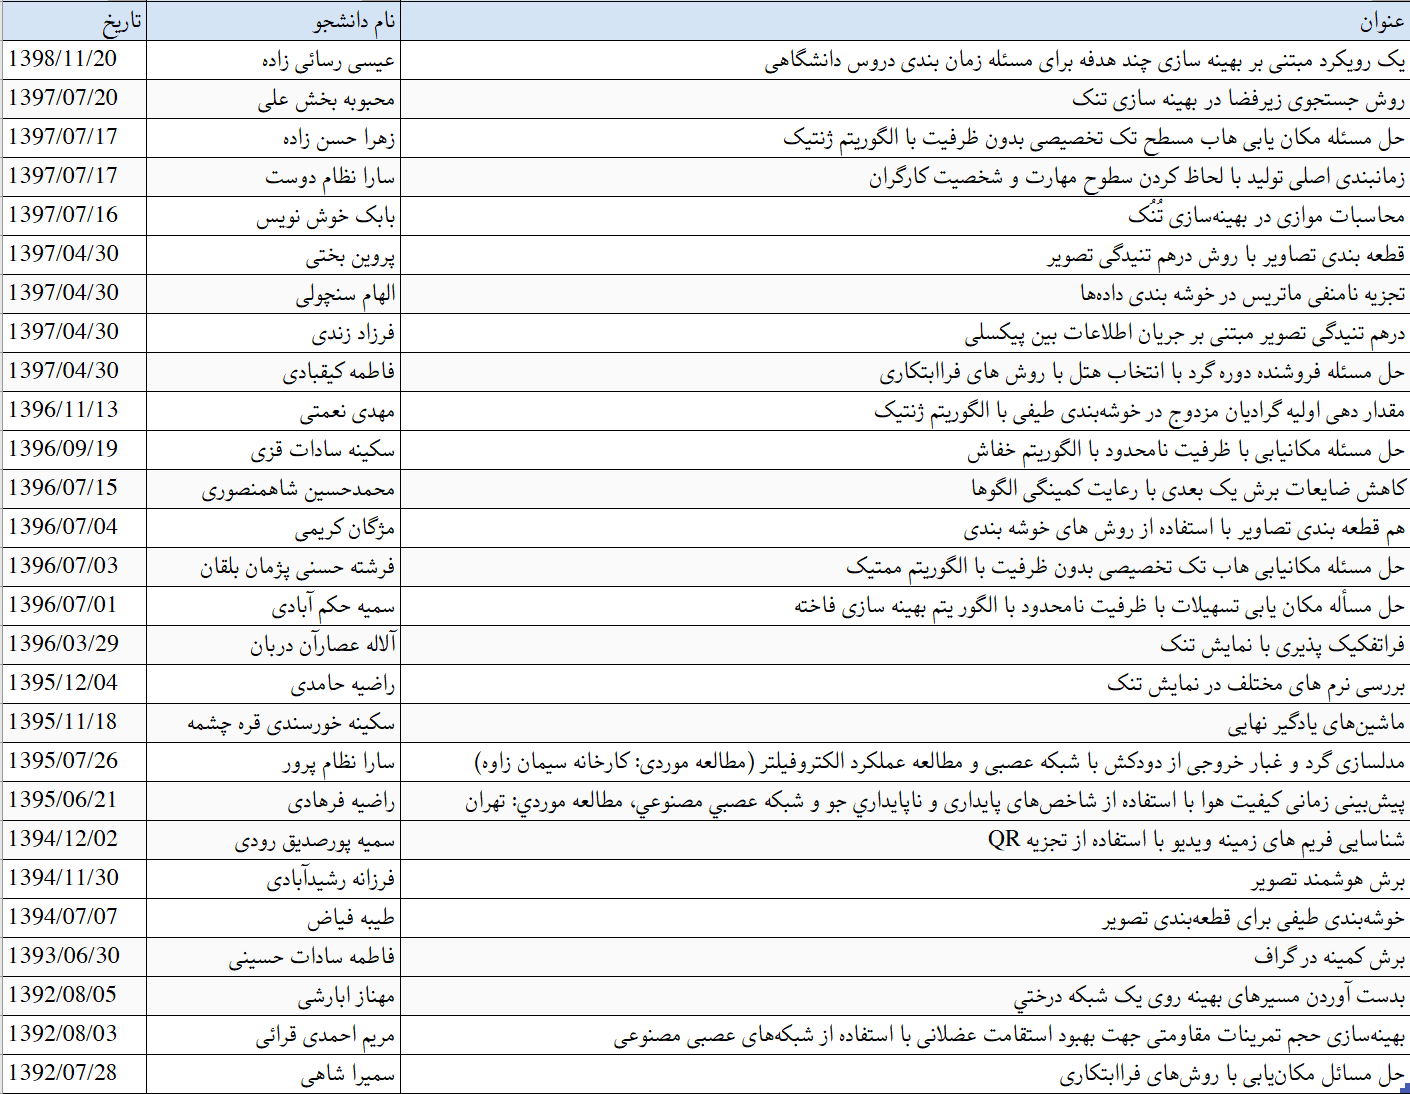
\includegraphics[width=1\linewidth]{MSc-Projects.png}

\end{document}
